% Heatmap visualization using TikZ and pgfplots
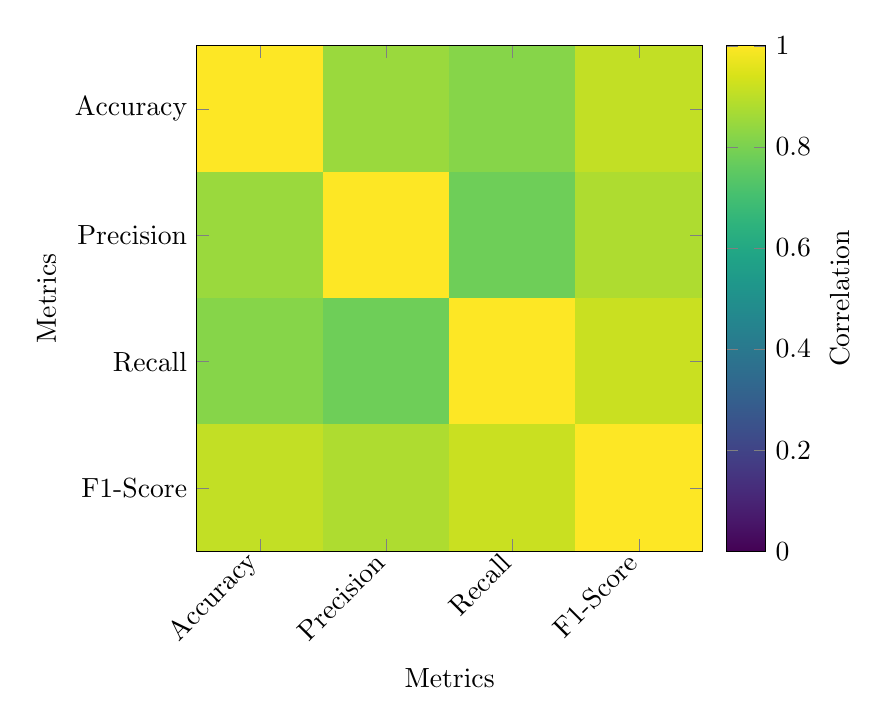
\begin{tikzpicture}
\begin{axis}[
    colormap/viridis,
    colorbar,
    colorbar style={
        ylabel={Correlation}
    },
    width=10cm,
    height=8cm,
    xlabel={Metrics},
    ylabel={Metrics},
    xticklabel style={rotate=45, anchor=east},
    yticklabel style={anchor=east},
    xtick=data,
    ytick=data,
    xticklabels={Accuracy, Precision, Recall, F1-Score},
    yticklabels={Accuracy, Precision, Recall, F1-Score},
    point meta min=0,
    point meta max=1,
    enlargelimits=false,
    axis equal image
]
\addplot[
    matrix plot,
    mesh/cols=4,
    point meta=explicit
] coordinates {
    (0,0) [1.00] (1,0) [0.85] (2,0) [0.82] (3,0) [0.91]
    (0,1) [0.85] (1,1) [1.00] (2,1) [0.78] (3,1) [0.88]
    (0,2) [0.82] (1,2) [0.78] (2,2) [1.00] (3,2) [0.92]
    (0,3) [0.91] (1,3) [0.88] (2,3) [0.92] (3,3) [1.00]
};
\end{axis}
\end{tikzpicture}
